\begin{frame}{Experiments}{Hexagon pattern}
  \small{
    \begin{enumerate}
    \item The number of robots $n=10,20,30,40$.
    \item For each $n$, run $10$ trials of simulations.
    \end{enumerate}
  }
  \only<1>{
    \centering
     \begin{figure}
      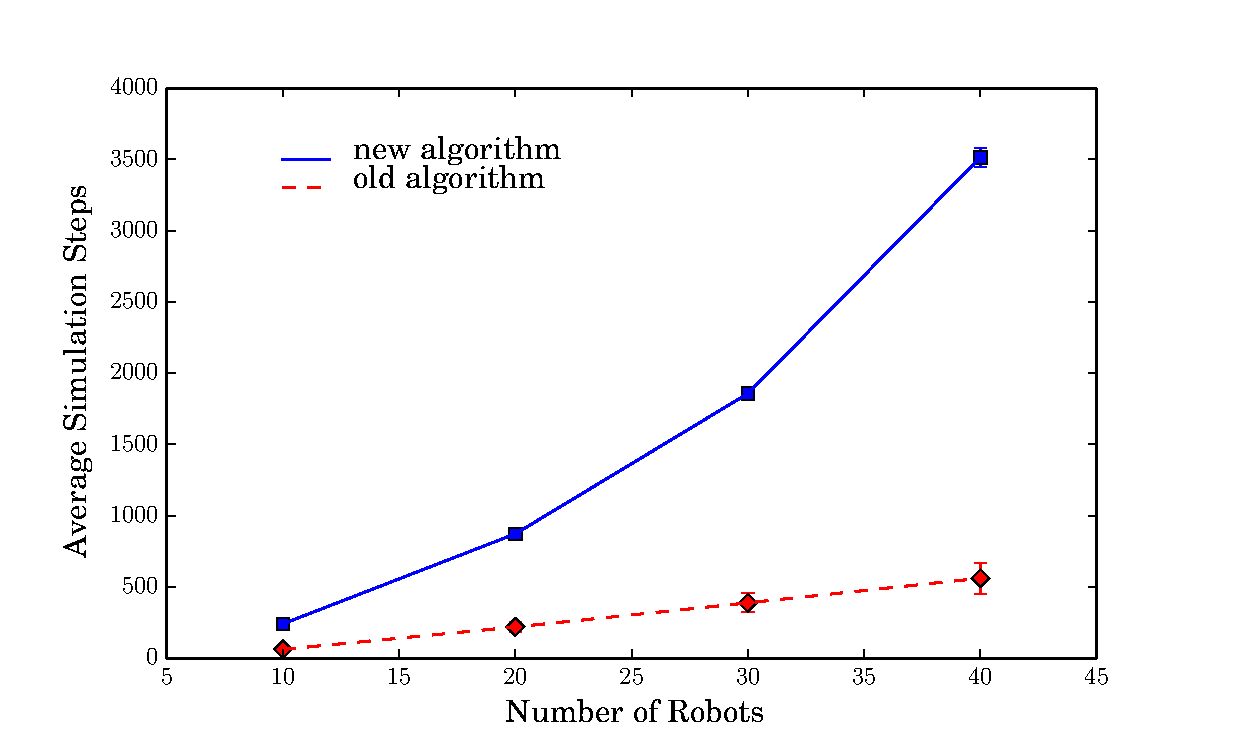
\includegraphics[width=0.65\textwidth]{figs/steps_hexagon}
     \end{figure}
    \small{Simulation Steps Comparison}
  }
  \only<2>{
    \centering
    \begin{figure}
      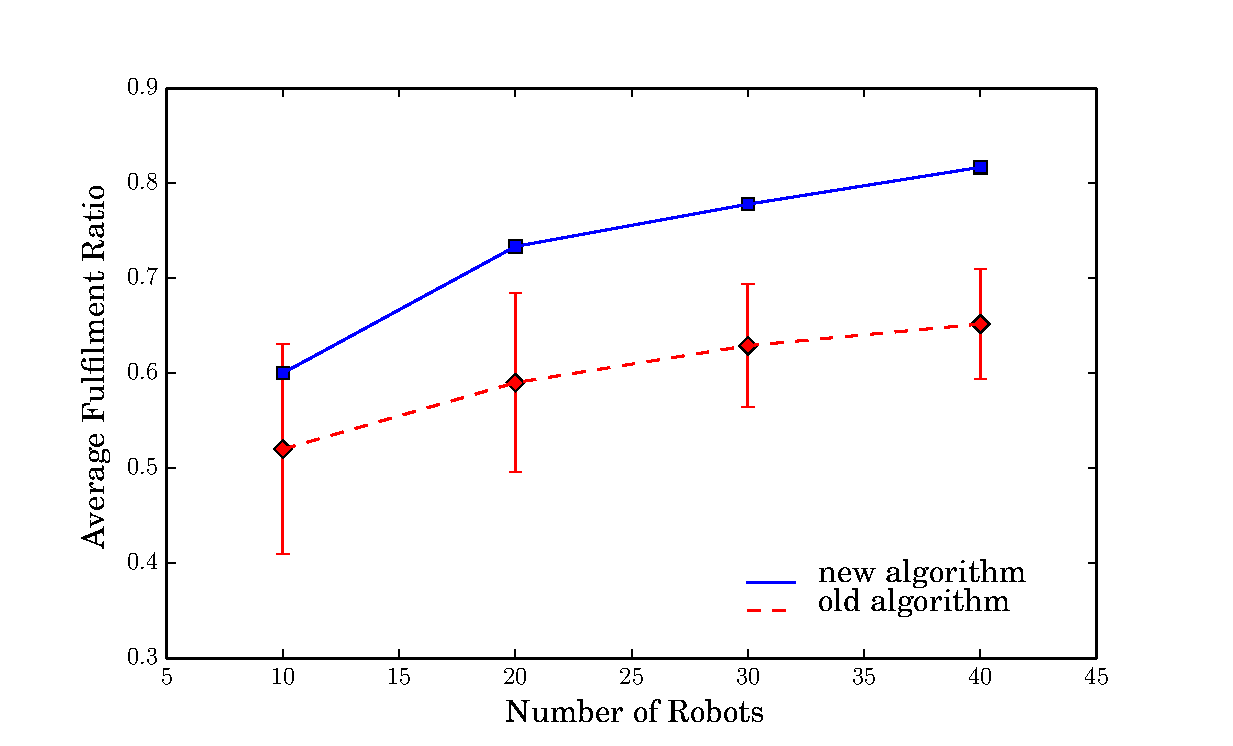
\includegraphics[width=0.65\textwidth]{figs/ratio_hexagon}
    \end{figure}
    \small{Simulation Quality Comparison}
  }
\end{frame}